\documentclass[tikz]{standalone}
\usepackage{pgfplots}
\usepgfplotslibrary{fillbetween}
\pgfplotsset{compat=newest}

\begin{document}
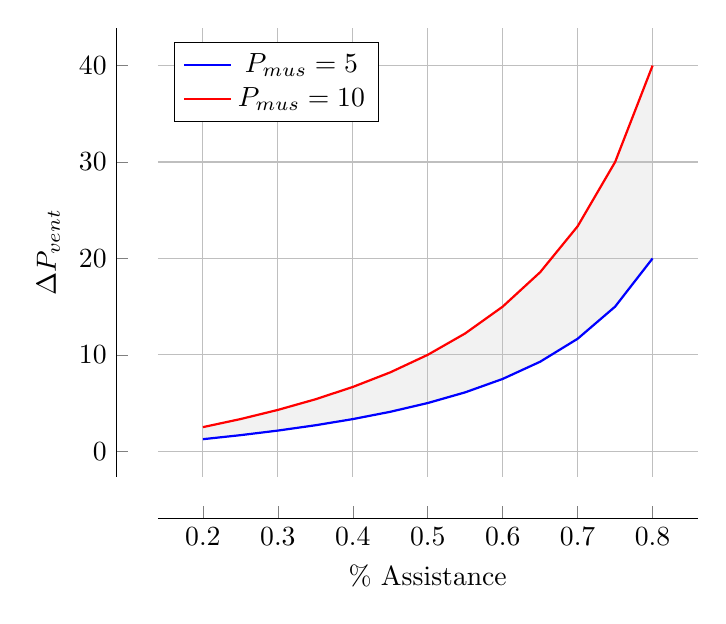
\begin{tikzpicture}

\begin{axis}[
    xlabel=\% Assistance,
    ylabel=$\Delta P_{vent}$,
    domain=.2:.8,
    axis lines*=left,
    axis line shift=15pt,
    legend pos=north west,
    grid=major,
]

\addplot+[name path=min, samples=13, thick, mark=none] {\x*5/(1-\x)};
\addplot+[name path=max, samples=13, thick, mark=none] {\x*10/(1-\x)};
\addplot  [lightgray, opacity=0.2] fill between [of=min and max];
\legend{$P_{mus}=5$,$P_{mus}=10$}

\end{axis}

\end{tikzpicture}
\end{document}
